\section{Probability Theory}
\label{sect:prob-theory}
\begin{enumerate}
\item Many topics in modern financial economics are built on \emph{stochastic
calculus}, which is touched upon in \Cref{sect:stochastic-calculus}. As
suggested by its name, it is a new type of calculus ``with randomness''; for
instance, rather than differentiating with respect to a deterministic time
variable, we differentiate with respect to a \emph{random variable} (you will
learn how to make sense of this in STAT3911).

Due to the probabilistic nature of stochastic calculus, having a solid
foundation in probability theory is critical for studying stochastic calculus
properly. Unfortunately, the probability knowledge from your first course in
probability is \emph{not} enough, so we will cover the basics of some more
advanced probability theory (known as the \emph{measure-theoretic} probability
theory) in \Cref{sect:prob-theory} and \Cref{sect:info-cond}. Next, armed with
these knowledge, we will start diving into the major sections in STAT3911,
which are more related to financial economics and hopefully more interesting
\faIcon[reuglar]{grin-wink}!

\end{enumerate}
\subsection{Set Theory Preliminaries}
\begin{enumerate}
\item \textbf{Set terminologies.} In the following, we will review
some terminologies about sets, which should be very familiar to you. Here, we
let \(\Omega\) be a nonempty \emph{universal} set (meaning that every set below
is a \emph{subset} of it).
\begin{center}
\begin{tabular}{lll}
\toprule
Name&Notation&Definition \\
\midrule
\makecell[l]{\(A\) is a subset of \(\Omega\), or \\
\(\Omega\) is a superset of \(A\)
}&
\makecell[l]{\(A\subseteq \Omega\), or \\
\(\Omega\supseteq A\)
}
&For all \(\omega\in A\), we have \(\omega\in\Omega\).  \\
\midrule
(Absolute) complement&\(A^c\)&\(\{\omega\in\Omega:\omega\notin A\}\) \\
Set difference&\(A\setminus B\)&\(A\cap B^c\) \\
Intersection (\(I\): index set)&\(\bigcap_{i\in I}A_i\)&\(\{\omega\in\Omega:\omega\in A_i\text{ for all \(i\in I\)}\}\) \\
Union &\(\bigcup_{i\in I}A_i\)&\(\{\omega\in\Omega:\omega\in A_i\text{ for some \(i\in I\)}\}\) \\
\midrule
Disjoint union &\(\biguplus_{i\in I}A_i\)&\makecell[l]{ meaning the same as \(\bigcup_{i\in I}A_i\),\\
 with the emphasis on the pairwise disjointness, \\
i.e., \(A_{i}\cap A_{j}=\varnothing\) for all \(i,j\in
I\) with \(i\ne j\).
}
 \\
\bottomrule
\end{tabular}
\end{center}
\item \textbf{Basic set properties.} You should be very familiar to the
following properties of sets (the sets below are arbitrary):
\begin{itemize}
\item \emph{Associativity of union and intersection:} \((A\cup B)\cup C=A\cup
(B\cup C)\) and \((A\cap B)\cap C=A\cap (B\cap C)\).
\item \emph{Commutativity of union and intersection:} \(A\cup B=B\cup A\) 
and \(A\cap B=B\cap A\).
\item \emph{De Morgan's laws:} \((\bigcup_{i\in I}A_i)^{c}=\bigcap_{i\in I}A_i^{c}\)
and \((\bigcap_{i\in I}A_i)^{c}=\bigcup_{i\in I}A_i^{c}\).
\end{itemize}
Make sure you are able to \emph{prove} these! (An useful way to prove a set
equality \(S=T\) is to prove (i) \(S\subseteq T\) and (ii) \(T\subseteq S\).)

\item\label{it:further-set-term} \textbf{Further set terminologies.} For the
following set theoretic terminologies, you may not have encountered them
before, so perhaps you should pay more attention here:
\begin{center}
\begin{tabular}{lll}
\toprule
Name&Notation&Definition \\
\midrule
\defn{Infimum (set)}&\(\inf_{k\ge n}A_k\)&\(\bigcap_{k\ge n}A_k\)\\
\defn{Supremum (set)}&\(\sup_{k\ge n}A_k\)&\(\bigcup_{k\ge n}A_k\) \\
\defn{Limit inferior (set)}&\(\liminf_{n\to\infty}A_n\)&\(\bigcup_{n=1}^{\infty}\bigcap_{k\ge n}A_k
=\sup_{n\ge 1}\inf_{k\ge n}A_k\)\\
\defn{Limit superior (set)}&\(\limsup_{n\to \infty}A_n\)&\(\bigcap_{n=1}^{\infty}\bigcup_{k\ge n}A_k
=\inf_{n\ge 1}\sup_{k\ge n}A_k\) \\
\defn{Limit of \(A_n\)}&\(A=\lim_{n\to \infty}A_n\) or \(A_n\to A\)&
\(\liminf_{n\to \infty}A_n=\limsup_{n\to\infty}A_n=A\) \\
\(\{A_n\}_{n\in\N}\) is \defn{increasing}&\(A_n\nearrow\)&\(A_1\subseteq A_2\subseteq\dotsb\) \\
\(\{A_n\}_{n\in\N}\) is \defn{decreasing}&\(A_n\searrow\)&\(A_1\supseteq A_2\supseteq\dotsb\) \\
\bottomrule
\end{tabular}
\end{center}
\item \textbf{Further set properties.} Here we will discuss some results about
the less familiar set terminologies from \labelcref{it:further-set-term}:
\begin{enumerate}
\item \label{it:liminfsup-interpret} \emph{(Interpreting limit inferior and limit superior)}
\begin{enumerate}
\item \(\liminf_{n\to \infty}A_n=\{\omega\in\Omega:\omega\in A_n\text{ for
\underline{a}ll \underline{b}ut \underline{f}initely \underline{m}any \(n\)}\}
=:\{\omega\in A_n\text{ abfm}\}\).
\item
\(\limsup_{n\to \infty}A_n=\{\omega\in\Omega:\omega\in A_n\text{ for infinitely many \(n\)}\}
=\{\omega\in\Omega:\omega\in A_n\text{ \underline{i}nfinitely \underline{o}ften}\}
=:\{\omega\in A_n\text{ io}\}\).
\end{enumerate}
\begin{pf}
\begin{enumerate}
\item Note that
\[
\liminf_{n\to \infty}A_n=\bigcup_{n=1}^{\infty}\bigcap_{k\ge n}A_k
=\{\omega\in\Omega:\exists n\in\N\text{ s.t. }\omega\in A_k\;\forall k\ge n\}
\]
and ``\(\exists n\in\N\text{ s.t. }\omega\in A_k\;\forall k\ge n\)'' just means
``\(\omega\in A_n\) for all but finitely many \(n\)'' in words.

\item Similar to above, and we can interpret ``\(\forall n\in\N\; \exists k\ge
n\text{ s.t. }\omega\in A_k\)'' as ``\(\omega\in A_n\) for infinitely many \(n\)''.
\end{enumerate}
\end{pf}
\item \label{it:liminfsup-relate} \emph{(Relating limit inferior and limit superior)}
\begin{enumerate}
\item \(\liminf_{n\to \infty}A_n\subseteq \liminf_{n\to \infty}A_n \).
\item \((\liminf_{n\to \infty}A_n)^{c}=\limsup_{n\to \infty}A_n^c \).
\item \((\limsup_{n\to \infty}A_n)^{c}=\liminf_{n\to \infty}A_n^c \).
\end{enumerate}
\begin{pf}
\begin{enumerate}
\item Because ``\(\omega\in A_n\) for all but finitely many \(n\)'' is just a
special case of ``\(\omega\in A_n\) for infinitely many \(n\)''.
\item Apply De Morgan's laws twice:
\[
\left(\liminf_{n\to \infty}A_n\right)^{c}
=\left(\bigcup_{n=1}^{\infty}\vc{\bigcap_{k\ge n}A_k}\right)^{c}
\overset{\text{DM}}{=} \bigcap_{n=1}^{\infty}\vc{\left(\bigcap_{k\ge n}A_k\right)^{c}}
\overset{\text{DM}}{=} \bigcap_{n=1}^{\infty}\left(\vc{\bigcup_{k\ge n}A_k^{c}}\right)
=\limsup_{n\to \infty}A_n^c .
\]
\item Again apply De Morgan's laws twice:
\[
\left(\limsup_{n\to \infty}A_n\right)^{c}
=\left(\bigcap_{n=1}^{\infty}\vc{\bigcup_{k\ge n}A_k}\right)^{c}
\overset{\text{DM}}{=} \bigcup_{n=1}^{\infty}\vc{\left(\bigcup_{k\ge n}A_k\right)^{c}}
\overset{\text{DM}}{=} \bigcup_{n=1}^{\infty}\left(\vc{\bigcap_{k\ge n}A_k^{c}}\right)
=\liminf_{n\to \infty}A_n^c .
\]
\end{enumerate}
\end{pf}
\item \label{it:lim-mono-sets} \emph{(Limits of monotone sequences of sets)}
\begin{enumerate}
\item If \(A_n\nearrow\), then \(\lim_{n\to \infty}A_n\) exists and equals \(\bigcup_{k=1}^{\infty} A_k\).

\begin{note}
Setting \(A_n:=\bigcup_{i=1}^{n}B_i\), since \(A_n\nearrow\), we can get the
intuitively appealing equality
\(\lim_{n\to\infty}\bigcup_{i=1}^{n}B_i=\bigcup_{i=1}^{\infty}B_i\), as \(\bigcup_{i=1}^{\infty}B_i
=\bigcup_{k=1}^{\infty}\left(\bigcup_{i=1}^{k}B_k\right).\)
\end{note}
\item If \(A_n\searrow\), then \(\lim_{n\to \infty}A_n\) exists and equals \(\bigcap_{k=1}^{\infty} A_k\).
\item For all collections \(\{A_n\}\subseteq\pow{\Omega}\), \(\liminf_{n\to \infty}A_n
=\lim_{n\to \infty}(\inf_{k\ge n}A_k)\) and \(\limsup_{n\to \infty}A_n
=\lim_{n\to \infty}(\sup_{k\ge n}A_k)\). \begin{note}
This explains the rationale behind the notations ``\(\liminf_{n\to
\infty}A_n\)'' and ``\(\limsup_{n\to \infty}A_n\)''.
\end{note}
\end{enumerate}
\begin{pf}
\begin{enumerate}
\item Assuming \(A_n\nearrow\), we have \vc{\(A_k\subseteq
\bigcap_{i=k}^{\infty}A_i\)}. Hence,
\[
\limsup_{n\to \infty}A_n=\bigcap_{n=1}^{\infty}\bigcup_{k=n}^{\infty}A_k
\subseteq \boxed{\bigcup_{k=1}^{\infty}\vc{A_k}}
\vc{\subseteq} \bigcup_{n=1}^{\infty}\vc{\bigcap_{i=k}^{\infty}A_i}
=\liminf_{n\to \infty}A_n
\subseteq \limsup_{n\to \infty}A_n.
\]
This forces \(\liminf_{n\to \infty}A_n=\limsup_{n\to
\infty}A_n=\bigcup_{k=1}^{\infty}A_k\), as desired.

\item Let \(B_n=A_n^c\) for all \(n\), then \(B_n\nearrow\). Applying (i), we
get
\[
\liminf_{n\to \infty}B_n
=\limsup_{n\to \infty}B_n
=\bigcup_{k=1}^{\infty}B_k.
\]
By \labelcref{it:liminfsup-relate}, we have \(\liminf_{n\to
\infty}B_n=(\limsup_{n\to \infty}A_n)^c\) and
\(\limsup_{n\to \infty}B_n=(\liminf_{n\to \infty}A_n)^c\). It then follows that
\[
\liminf_{n\to \infty}A_n=\limsup_{n\to \infty}A_n=\left(\bigcup_{k=1}^{\infty}B_k\right)^c
=\bigcap_{k=1}^{\infty}A_k^{c}.
\]
\item Note that \(\inf_{k\ge n}A_k\nearrow\) and \(\sup_{k\ge n}A_k\searrow\).
Hence,
\[
\liminf_{n\to \infty}A_n=\bigcup_{n=1}^{\infty}\bigcap_{k=n}^{\infty}A_k
=\bigcup_{n=1}^{\infty}\inf_{k\ge n}A_k
\overset{\text{(i)}}{=}\lim_{n\to \infty}\left(\inf_{k\ge n}A_k\right)
\]
and
\[
\limsup_{n\to \infty}A_n=\bigcap_{n=1}^{\infty}\bigcup_{k=n}^{\infty}A_k
=\bigcap_{n=1}^{\infty}\sup_{k\ge n}A_k
\overset{\text{(ii)}}{=}\lim_{n\to \infty}\left(\sup_{k\ge n}A_k\right).
\]
\end{enumerate}
\end{pf}
\end{enumerate}
\item \textbf{Indicator functions.} You should have learnt what an indicator
function is in your first probability course. This function continues to be of
great use here, so let us review it a bit.
\begin{itemize}
\item The \emph{indicator function} of \(A\subseteq \Omega\) is given by
\[
\indic_{A}(\omega)=\begin{cases}
1&\text{if \(\omega\in A\),} \\
0&\text{otherwise.} \\
\end{cases}
\]
\item Property: \(\indic_{A}\le\indic_{B}\) (i.e.,
\(\indic_{A}(\omega)\le\indic_{B}(\omega)\) for all \(\omega\in\Omega\)) iff
\(A\subseteq B\).
\end{itemize}
Indicator function can be applied for describing \(\limsup_{n\to \infty}A_n\)
and \(\liminf_{n\to \infty}A_n\):
\[
\limsup_{n\to \infty}A_n
=\left\{\omega\in\Omega:\sum_{n=1}^{\infty}\indic_{A_n}(\omega)=\infty\right\}
,\quad
\liminf_{n\to \infty}A_n
=\left\{\omega\in\Omega:\sum_{n=1}^{\infty}\indic_{A_{n}^{\rc{c}}}(\omega)<\infty\right\}.
\]
This is because when \(\omega\in A_n\) infinitely often, infinitely many
\(\indic_{A_n}(\omega)\) would equal one; when \(\omega\in A_n\) for all but
finitely many \(n\), finitely many \(\indic_{A_n^{\rc{c}}}(\omega)\) would
equal one.

\item \textbf{Images and preimages.} A pair of concepts that will frequently
appear in our discussion of measure theoretic probability theory is
\emph{image} and \emph{preimage}, which is covered in MATH2012.

Let \(\Omega\) and \(\Omega'\) be two sets, and \(X:\Omega\to\Omega'\) be a
function.  The \emph{image} of \(A\subseteq \Omega\) under \(X\) is
\(X(A):=\{X(\omega):\omega\in A\}\), and the \emph{preimage} of \(A'\subseteq
\Omega'\) under  is \(X^{-1}(A'):=\{\omega\in\Omega:X(\omega)\in A'\}\).
\begin{center}
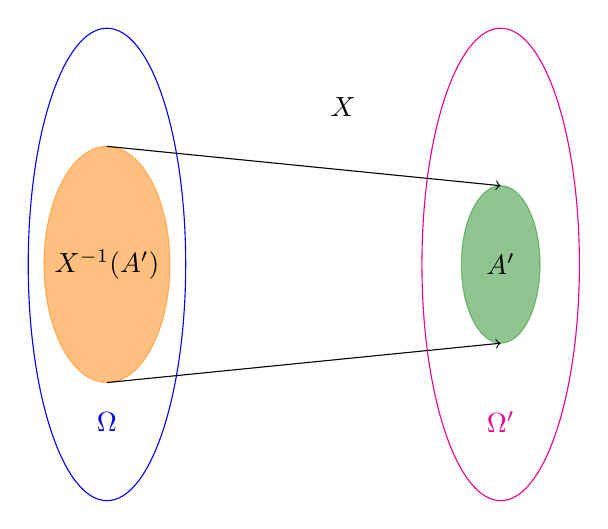
\begin{tikzpicture}
\draw[blue] (0,0) ellipse [x radius=1cm, y radius=3cm];
\draw[magenta] (5,0) ellipse [x radius=1cm, y radius=3cm];
\draw[ForestGreen, fill, opacity=0.5] (5,0) ellipse [x radius=0.5cm, y radius=1cm];
\draw[orange, fill, opacity=0.5] (0,0) ellipse [x radius=0.8cm, y radius=1.5cm];
\draw[->] (0,1.5) -- (5,1);
\draw[->] (0,-1.5) -- (5,-1);
\node[] () at (0,0) {\(X^{-1}(A')\)};
\node[] () at (5,0) {\(A'\)};
\node[] () at (3,2) {\(X\)};
\node[blue] () at (0,-2) {\(\Omega\)};
\node[magenta] () at (5,-2) {\(\Omega'\)};
\end{tikzpicture}
\end{center}
Let \(\mathcal{A}'\) be a family/set of sets in \(\Omega'\) (i.e., a
subfamily/subset of \(\mathcal{P}(\Omega')\). Then, the notation
\(X^{-1}(\mathcal{A}')\) refers to the family/set of all preimages of sets in
\(\mathcal{A}\), i.e., \(\{X^{-1}(A'):A'\in\mathcal{A}'\}\).
\item\label{it:preimg-prop} \textbf{Properties of preimages.} Let \(A',B'\)
denote any subsets of \(\Omega'\), and \(\{A_i'\}_{i\in I}\) be any
subcollection in \(\mathcal{P}(\Omega')\).
\begin{enumerate}
\item \emph{(preservation of complementation)} \(\big(X^{-1}(A')\big)^{c}=X^{-1}(A'^{c})\).
\item \emph{(preservation of union)} \(X^{-1}(\bigcup_{i\in I}A_i')=\bigcup_{i\in I}X^{-1}(A_i')\).
\item \emph{(preservation of intersection)} \(X^{-1}(\bigcap_{i\in I}A_i')=\bigcap_{i\in I}X^{-1}(A_i')\).
\item \emph{(monotonicity)} Let \(\mathcal{A}',\mathcal{B}'\subseteq
\mathcal{P}(\Omega')\). Then, \(\mathcal{A}'\subseteq \mathcal{B}'\implies
X^{-1}(\mathcal{A}')\subseteq X^{-1}(\mathcal{B}')\).
\end{enumerate}
\begin{pf}
We demonstrate the proof for (b) and (d) here and leave the rest as exercises.

\begin{enumerate}
\item[(b)]
``\(\subseteq\)'': Fix any \(\omega\in X^{-1}(\bigcup_{i\in I}A_i')\). By
definition, \(X(\omega)\in\bigcup_{i\in I}A_i'\), thus there exists some \(i\in
I\) such that \(X(\omega)\in A_i'\), or \(\omega\in X^{-1}(A_i')\). This means
\(\omega\in \bigcup_{i\in I}X^{-1}(A_i')\).

``\(\supseteq\)'': Highly similar to ``\(\subseteq\)''; just work backward.

\item[(d)] Assume \(\mathcal{A}'\subseteq \mathcal{B}'\). Now, fix any \(A\in
X^{-1}(\mathcal{A}')\). By definition, we have \(A=X^{-1}(A')\) for some
\(A'\in\mathcal{A}'\). Since \(\mathcal{A}'\subseteq \mathcal{B}'\), we also
have \(A'\in\mathcal{B}'\), meaning that
\(A\in\{X^{-1}(A'):A'\in\mathcal{B}'\}=X^{-1}(\mathcal{B}')\).
\end{enumerate}
\end{pf}
\end{enumerate}
\subsection{Probability Spaces}
\begin{enumerate}
\item \textbf{Systems of sets.} \emph{Systems of sets} are utilized for
constructing families of ``selected'' sets on which a probability measure
\(\pr\) can be defined consistently without having any issue. It turns out that
there are indeed some sets to which we cannot assign any reasonable
probability, like \emph{Vitali set} \warn{} (see STAT7610 for more details), so
in general we cannot just blindly choose the whole power set of sample space as
the domain of the probability measure \(\pr\) (though it is quite tempting!),
and we need to exclude those ``pathological'' sets by restricting the domain
\warn{}. \begin{note}
However, such issues only arise when the sample space \(\Omega\) is
uncountable. If \(\Omega\) is countable, then we can define \(\pr\) on the
power set \(\mathcal{P}(\Omega)\) without issues.
\end{note}

There are multiple systems of sets here,
but they all share a common theme, which is about constructing a family of
sets that is \emph{closed} under certain set operations, i.e., performing
these operations on sets in \(\mathcal{F}\) would not yield something outside
\(\mathcal{F}\) --- being ``stable'' in some sense.  Intuitively, we are
interested in this kind of properties because they can make the families
of sets ``rich enough'', in the sense that the families contain ``sufficiently
many well-behaved sets''. Here, we will discuss two types of systems of sets:
(i) algebra and (ii) \ystar{} \(\sigma\)-algebra (important concept for
probability theory!)

\item \textbf{Definitions of algebra and \(\sigma\)-algebra.}
\begin{itemize}
\item A family \(\mathcal{F}\subseteq \pow{\Omega}\) is an \defn{algebra} (or
\defn{field}) on \(\Omega\) if
\begin{enumerate}[label={(\arabic*)}]
\item \(\varnothing\in\mathcal{F}\).
\item \emph{(closed under complementations)} \(A\in\mathcal{F}\implies A^c=\Omega\setminus A\in\mathcal{F}\).
\item \emph{(closed under unions)}
\(A,B\in\mathcal{F}\implies A\cup B\in\mathcal{F}\).
\end{enumerate}
\item \ystar{} A family \(\mathcal{F}\subseteq \pow{\Omega}\) is a
\defn{\(\sigma\)-algebra} (or \defn{\(\sigma\)-field}) on \(\Omega\) if
\begin{enumerate}[label={(\arabic*)}]
\item \(\varnothing\in\mathcal{F}\).
\item \emph{(closed under complementations)} \(A\in\mathcal{F}\implies A^c=\Omega\setminus A\in\mathcal{F}\).
\item \emph{(closed under countable unions)}
\(A_1,A_2,\dotsc\in\mathcal{F}\implies \bigcup_{i=1}^{\infty}A_i\in\mathcal{F}\).
\end{enumerate}
\begin{note}
A \(\sigma\)-algebra is actually also closed under several more set operations,
e.g., finite unions, finite/countable intersections, and set differences:
\begin{itemize}
\item \emph{finite intersections:}
It follows from the closedness under countable unions from setting
\(A_{n+1}=A_{n+2}=\dotsb=\varnothing\), because
\(\bigcup_{i=1}^{n}A_i=\bigcup_{i=1}^{\infty}A_i\) in this case.

\item \emph{countable intersections:}
To show this, we can use De Morgan law, and the
closedness under countable unions and complementations:
\[
A_1,A_2,\dotsc\in\mathcal{F}
\implies \bigcap_{i=1}^{\infty}A_i\overset{\text{DM}}{=}
\left(\bigcup_{i=1}^{\infty}A_i^{c}\right)^{c}
\in\mathcal{F}.
\]
\item \emph{finite intersections:}
It follows from the closedness under countable intersections from setting
\(A_{n+1}=A_{n+2}=\dotsb=\Omega\), because
\(\bigcap_{i=1}^{n}A_i=\bigcap_{i=1}^{\infty}A_i\) in this case.

\item \emph{set differences:} 
Fix any \(A,B\in\mathcal{F}\). Then \(B^c\in\mathcal{F}\). Applying the
closedness under finite intersections, we have \(A\setminus B=A\cap
B^c\in\mathcal{F}\).
\end{itemize}
\end{note}
\end{itemize}
\item \textbf{Examples of \(\sigma\)-algebras.}
\begin{enumerate}[label={(\arabic*)}]
\item The \defn{trivial \(\sigma\)-algebra} on \(\Omega\) is
\(\mathcal{F}=\{\varnothing,\Omega\}\).
\begin{note}
It is the \emph{smallest} \(\sigma\)-algebra on \(\Omega\), i.e., every
\(\sigma\)-algebra on \(\Omega\) is a superset of the trivial
\(\sigma\)-algebra.  This is because containing \(\varnothing\) and being
closed under complementations would force a \(\sigma\)-algebra to at least
contain \(\varnothing\) and \(\Omega\).
\end{note}

\item The power set \(\mathcal{F}=\mathcal{P}(\Omega)\) is a \(\sigma\)-algebra
on \(\Omega\).

\begin{remark}
\item It is a \(\sigma\)-algebra on \(\Omega\) because complement of subset of \(\Omega\) is still a subset of \(\Omega\), and countable union of subsets of \(\Omega\) is still a subset of \(\Omega\).
\item It is the \emph{largest} \(\sigma\)-algebra on \(\Omega\), i.e., every
\(\sigma\)-algebra on \(\Omega\) is a subset of \(\mathcal{P}(\Omega)\) (which
follows from definition).
\end{remark}
\end{enumerate}
\item \textbf{\(\sigma\)-algebra generated by a family of sets.}
Let us motivate this concept by considering some examples of constructing
\(\sigma\)-algebras from sets:
\begin{itemize}
\item \emph{Constructing from one set:} Start with a set \(A\subseteq \Omega\).
Then consider the following two sets that partition \(\Omega\):
\[
A\qquad A^c
\]
By putting zero/one/two of them into an union, we can get 4 combinations:
\begin{itemize}
\item \emph{zero:} \(\varnothing\)
\item \emph{one:} \(A\), \(A^c\)
\item \emph{two:} \(A\cup A^c=\Omega\)
\end{itemize}
These four sets form a \(\sigma\)-algebra: \(\{\varnothing, A, A^c, \Omega\}\).
\item \emph{Constructing from two sets:} Here we start with two sets
\(A,B\subseteq \Omega\). Then consider the following \(2^2=4\) sets that
partition \(\Omega\): \(A\cap B\), \(A^c\cap B\), \(A\cap B^c\), and \(A^c\cap
B^c\).
\begin{center}
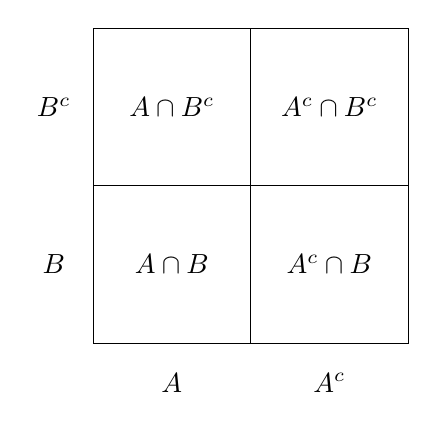
\begin{tikzpicture}
\draw[] (0,0) rectangle (2,2);
\draw[] (0,4) rectangle (2,2);
\draw[] (4,0) rectangle (2,2);
\draw[] (2,2) rectangle (4,4);
\node[] () at (1,-0.5) {\(A\)};
\node[] () at (3,-0.5) {\(A^c\)};
\node[] () at (-0.5,1) {\(B\)};
\node[] () at (-0.5,3) {\(B^{c}\)};
\node[] () at (1,1) {\(A\cap B\)};
\node[] () at (3,1) {\(A^c\cap B\)};
\node[] () at (1,3) {\(A\cap B^c\)};
\node[] () at (3,3) {\(A^c\cap B^c\)};
\end{tikzpicture}
\end{center}
By putting zero/one/two/three/four of them into an union, we can get \(\binom{4}{0}+\binom{4}{1}+\binom{4}{2}+\binom{4}{3}+\binom{4}{4}=(1+1)^4=16\) combinations:
\begin{itemize}
\item \emph{zero:} \(\varnothing\)
\item \emph{one:} \(A\cap B\), \(A^c\cap B\), \(A\cap B^c\), \(A^c\cap B^c\)
\item \emph{two:}
\begin{itemize}
\item \(B=(A\cap B)\cup(A^c\cap B)\)
\item \(A=(A\cap B)\cup(A\cap B^c)\)
\item \((A\cap B)\cup (A^c\cap B^c)\)
\item \((A^c\cap B)\cup(A\cap B^c)\)
\item \(A^c=(A^c\cap B)\cup(A^c\cap B^c)\)
\item \(B^c=(A\cap B^c)\cup(A^c\cap B^c)\)
\end{itemize}
\item \emph{three:} (just complement of each of the four sets in the partition indeed)
\begin{itemize}
\item \(A^c\cup B^c=(A\cap B)^c\)
\item \(A\cup B^c=(A^c\cap B)^c\)
\item \(A^c\cup B=(A\cap B^c)^c\)
\item \(A\cup B=(A^c\cap B^c)^c\)
\end{itemize}
\item \emph{four:} \(\Omega\)
\end{itemize}
These 16 sets form a \(\sigma\)-algebra.
\end{itemize}

The \(\sigma\)-algebras above are indeed examples of \(\sigma\)-algebra
\emph{generated by a family of sets}. The one-set example is the
\(\sigma\)-algebra generated by the family \(\mathcal{A}=\{A\}\), and the two-set example
is the \(\sigma\)-algebra generated by the family \(\mathcal{A}=\{A,B\}\).

In general, let \(\mathcal{A}\) be a family of sets in \(\Omega\). Then the
\defn{\(\sigma\)-algebra generated by \(\mathcal{A}\)}, denoted by
\(\sigma(\mathcal{A})\), is the \emph{smallest} \(\sigma\)-algebra that
contains every set in the family \(\mathcal{A}\), i.e., (i)
\(\sigma(\mathcal{A})\) is a \(\sigma\)-algebra on \(\Omega\) that contains
\(\mathcal{A}\), and (ii) for every \(\sigma\)-algebra \(\mathcal{F}'\) on
\(\Omega\) with \(\vc{\mathcal{A}}\subseteq \mathcal{F}'\), we have
\(\sigma(\vc{\mathcal{A}})\subseteq \mathcal{F}'\).
We consider the smallest one here so
that all ``irrelevant'' sets are excluded in the \(\sigma\)-algebra.

\item \textbf{Borel \(\sigma\)-algebra.} Next, we shall consider a commonly
used \(\sigma\)-algebra that contains most sets (subsets of \(\R\)) we can
imagine, called \emph{Borel \(\sigma\)-algebra} (it is difficult to think of a
set that is not in this \(\sigma\)-algebra!).

The \defn{Borel \(\sigma\)-algebra on \(\R\)}, denoted by \(\mathcal{B}(\R)\)
or \(\mathcal{B}\), is the \(\sigma\)-algebra generated by the family
\(\mathcal{A}=\{(a,b]:a<b\}\) of left-open and right-closed intervals, i.e.,
\(\mathcal{B}=\sigma(\mathcal{A})\). Every set in \(\mathcal{B}\) is said to be
a \defn{Borel set}.

To see why \(\mathcal{B}\) includes most subsets of \(\R\) we can imagine, let
us explore what types of subsets of \(\R\) are included in \(\mathcal{B}\):
\begin{itemize}
\item \emph{singletons:} \(\bigcap_{i=1}^{\infty}(a-1/i,a]=\{a\}\in\mathcal{B}\)
\item \emph{closed intervals:} \((a,b]\cup\{a\}=[a,b]\in\mathcal{B}\)
\item \emph{open intervals:} \((a,b]\setminus \{a\}=(a,b)\in\mathcal{B}\)
\item \emph{left-closed and right-open intervals:} \([a,b]\setminus
\{b\}=[a,b)\in\mathcal{B}\)
\item any finite/countable union(s)/intersection(s) of (complement) of sets in
the types above belongs to \(\mathcal{B}\)
\end{itemize}
As you can see, it is rather difficult (but not impossible!) to think of a
subset of \(\R\) that is in none of the types above.

\item \textbf{\(\sigma\)-algebra on subset of \(\R\).} It turns out that Borel
\(\sigma\)-algebra can be defined in a more general fashion, and the Borel
\(\sigma\)-algebra on \(\R\) is just a special case; see STAT7610 for more
details. Generally, a Borel \(\sigma\)-algebra on \(A\subseteq \R\) can be
obtained by \(\mathcal{B}(A)=\sigma(\{(a,b]\cap A:a<b\})\). For example, the
Borel \(\sigma\)-algebra on \([0,1]\) is given by
\(\mathcal{B}([0,1])=\sigma(\{(a,b]:0\le a< b\le 1\})\).

\item \textbf{Probability measures.} With the knowledge of \(\sigma\)-algebra,
we can define probability measure formally (the definition of probability
measure you have seen previously is perhaps informal). Let \(\Omega\) be a
sample space and \(\mathcal{F}\) be a \(\sigma\)-algebra on \(\Omega\). Then, a
\defn{probability measure} \(\pr\) on \(\mathcal{F}\) (or on
\((\Omega,\mathcal{F})\), which is known as a \defn{measurable space}) is a
real-valued function on \(\mathcal{F}\) satisfying:
\begin{enumerate}[label={(\arabic*)}]
\item \emph{(nonnegativity)} \(\prob{A}\ge 0\) for all \(A\in\mathcal{F}\).
\item \emph{(unitarity)} \(\prob{\Omega}=1\).
\item \emph{(countable additivity)}
\(A_1,A_2,\dotsc\in\mathcal{F}\text{ pairwise disjoint}
\implies \prob{\biguplus_{i=1}^{\infty}A_i}=\sum_{i=1}^{\infty}\prob{A_i}\).
\end{enumerate}
\begin{remark}
\item Informally, countable additivity allows us to ``pull \(\biguplus\) out of
\(\mu\) and make it \(\sum_{}^{}\)'' (explaining why there is a
``\(+\)'' in the notation ``\(\biguplus\)'').
\item \emph{(probability of empty set)} By taking \(A_1=\Omega\) and
\(A_2=A_3=\dotsb=\varnothing\), from countable additivity we know
\(1=\prob{\Omega}=\prob{\biguplus_{i=1}^{\infty}A_i}
=\sum_{i=1}^{\infty}\prob{A_i}=\prob{\Omega}+\sum_{i=2}^{\infty}\prob{\varnothing}
\), which implies \(\sum_{i=2}^{\infty}\prob{\varnothing}=0\). This forces
\(\prob{\varnothing}=0\), as expected.
\item \emph{(finite additivity)} By taking
\(A_{n+1}=A_{n+2}=\dotsb=\varnothing\), we can show also the \emph{finite
additivity}: \(A_1,\dotsc,A_n\in\mathcal{F}\text{ pairwise disjoint}\implies
\prob{\biguplus_{i=1}^{n}A_i}=\sum_{i=1}^{n}\prob{A_i}\).
\end{remark}
These three defining properties of a probability measure are sometimes known as
the \defn{probability axioms}. Every set in \(\mathcal{F}\) is called an
\defn{event}. The triple \((\Omega,\mathcal{F},\pr)\) is called a
\defn{probability space}. \begin{note} If we replace \(\pr\) by a
\emph{measure} in general\footnote{As we are primarily focusing on probability
measures, we omit the definition of a general measure here; see STAT7610 for
more details.} (e.g., Lebesgue measure, which corresponds to usual notions of
``length'', ``area'', ``volume'', etc.), then the triple is called a
\defn{measure space}.
\end{note}

\item \label{it:prob-meas-prop} \textbf{Properties of probability measures.}
Based on the three probability axioms, we can deduce many properties of
probability which may be familiar to you. In the following, let \(A\), \(B\),
and \(A_i\)'s be sets in \(\mathcal{F}\).
\begin{enumerate}
\item \emph{(subtractivity)} If \(A\subseteq B\), then \(\prob{B\setminus A}=\prob{B}-\prob{A}\).
\item \emph{(monotonicity)} \(A\subseteq B\implies \prob{A}\le\prob{B}\).
\item \emph{(complement)} \(\prob{A^c}=1-\prob{A}\).
\item \emph{(\(\text{union}+\text{intersection}=\text{individual sum}\))}
\(\prob{A\cup B}+\prob{A\cap B}=\prob{A}+\prob{B}\).
\item \emph{(interchanging limit and probability)}
If \(A_n\nearrow\) or \(A_n\searrow\), then \(\lim_{n\to\infty}\prob{A_n}=\prob{\lim_{n\to\infty}A_n}\).
\begin{note}
We have \(A_1,A_2,\dotsc\in\mathcal{F}\implies
\lim_{n\to\infty}A_n\in\mathcal{F}\) as we can write
\(\lim_{n\to\infty}A_n=\bigcup_{n=1}^{\infty}\bigcap_{k\ge n}^{}A_k\), which is
a \emph{countable} union of \emph{countable} intersections of sets in
\(\mathcal{F}\), thus it is in \(\mathcal{F}\).
\end{note}
\item \emph{(countable subadditivity)} \(\prob{\bigcup_{i=1}^{\infty}A_i}\le\sum_{i=1}^{\infty}\prob{A_i}\).
\begin{note}
By setting \(A_{n+1}=A_{n+2}=\dotsb=\varnothing\), we can obtain \emph{finite
subadditivity}: \(\prob{\bigcup_{i=1}^{n}A_i}\le\sum_{i=1}^{n}\prob{A_i}\).
\end{note}
\end{enumerate}
\begin{pf}
\begin{enumerate}
\item It follows from the finite additivity since \(A\) and \(B\setminus A\)
are pairwise disjoint.
\item By subtractivity, we have
\(\prob{A}=\prob{B}-\underbrace{\prob{B\setminus A}}_{\ge 0}\le\prob{B}\).
\item It follows from setting \(B=\Omega\) in the set difference property.
\item The trick is to write \(A\cup B=A\uplus (B\setminus A)=A\uplus (B\setminus
(A\cap B))\), and thus by finite additivity and subtractivity we have
\[\prob{A\cup B}=\prob{A}+\vc{\prob{B\setminus(A\cap B)}}
=\prob{A}+\vc{\prob{B}-\prob{A\cap B}}.
\]
Rearranging this gives the desired result.

\item First consider the case with \(A_n\nearrow\). Let \(B_1:=A_1\) and
\(B_n:=A_n\setminus A_{n-1}\) for every integer \(n\ge 2\). By construction,
\(B_n\)'s are pairwise disjoint, and
\(A_n=\bigcup_{i=1}^{n}A_i=\biguplus_{i=1}^{n}B_i\) for every \(n\in\N\). We
then have \(\bigcup_{i=1}^{\infty}A_i=\lim_{n\to\infty}\bigcup_{i=1}^{n}A_i
=\lim_{n\to\infty}\biguplus_{i=1}^{n}B_i=\biguplus_{i=1}^{\infty}B_i\), and thus
\begin{align*}
\prob{\lim_{n\to \infty}A_n}
&\overset{\text{\labelcref{it:lim-mono-sets}}}{=}
\prob{\bigcup_{i=1}^{\infty}A_i}
=\prob{\biguplus_{i=1}^{\infty}B_i}
=\sum_{i=1}^{\infty}\prob{B_i}
=\lim_{n\to\infty}\sum_{i=1}^{n}\prob{B_i} \\
&=\lim_{n\to\infty}\prob{\biguplus_{i=1}^{n}B_i}
=\lim_{n\to\infty}\prob{A_n}.
\end{align*}
For the other case with \(A_n\searrow\), observe that \(A_n^c\nearrow\), and we
have \(\lim_{n\to\infty}A_n^c=(\lim_{n\to\infty}A_n)^{c}\) by
\labelcref{it:liminfsup-relate}. Therefore,
\begin{align*}
\prob{\lim_{n\to\infty}A_n}
&=1-\prob{\left(\lim_{n\to\infty}A_n\right)^{c}}
=1-\prob{\lim_{n\to\infty}A_n^{c}}
\overset{\text{proven}}{=}
1-\lim_{n\to\infty}\prob{A_n^c} \\
&=\lim_{n\to\infty}(1-\prob{A_n^{c}})
=\lim_{n\to\infty}\prob{A_n}.
\end{align*}
\item  Let \(B_1:=A_1\) and \(B_n:=A_n\setminus \bigcup_{i=1}^{n-1}A_i\) for
every integer \(n\ge 2\).  Then by construction, (i) \(B_n\)'s are pairwise
disjoint, (ii) \(B_n\subseteq A_n\) for every \(n\in\N\), and (iii)
\(\bigcup_{i=1}^{n}A_i=\biguplus_{i=1}^{n}B_i\) for every \(n\in\N\).

By (iii), we have \(\bigcup_{i=1}^{\infty}A_i
=\lim_{N\to\infty}\bigcup_{i=1}^{N}A_i =\lim_{N\to\infty}\biguplus_{i=1}^{N}B_i
=\biguplus_{i=1}^{\infty}B_i \). Thus,
\[
\mu\left(\bigcup_{i=1}^{\infty}A_i\right)
=\mu\left(\biguplus_{i=1}^{\infty}B_i\right)
=\sum_{i=1}^{\infty}\mu(B_i)
\overset{\text{(ii), monotonicity}}{\le}\sum_{i=1}^{\infty}\mu(A_i).
\]
\end{enumerate}
\end{pf}
\end{enumerate}
\subsection{Random Variables}
\label{subsect:random-var}
\begin{enumerate}
\item In your first course in probability, you should have learnt that a random
variable is a function from the sample space \(\Omega\) to \(\R\): It
quantifies each sample point \(\omega\) in the sample space.  However, this
``definition'' is indeed an informal one, and actually an extra condition is
needed, namely \emph{measurability}.

A function \(X:\Omega\to\R\) is a \defn{(\vc{\(\mathcal{F}\)}-)random variable}
if \(X^{-1}(\mathcal{B})=\{X^{-1}(B):B\in\mathcal{B}\}\subseteq
\vc{\mathcal{F}}\), where \(\mathcal{B}\) is the Borel \(\sigma\)-algebra on
\(\R\).
\begin{note}
In some contexts, we may implicitly adapt the definition a bit by replacing
\(\R\) by \(\eR=[-\infty,\infty]\), the set of extended real numbers.  In
respond to this change, we would change \(\mathcal{B}\) to the Borel
\(\sigma\)-algebra on \(\eR\), which is given by \(\{B\cup E:B\in\mathcal{B},
E\in\{-\infty,\infty\}\}\).
\end{note}

Recall that the probability \(\prob{X\in B}\) is indeed given by
\(\prob{\{\omega\in\Omega:X(\omega)\in B\}}=\prob{X^{-1}(B)}\). So the idea of
this extra condition is to ensure that for all sets of practical interest (the
Borel sets), it is possible to compute \(\prob{X\in B}\). In other words, we
need to require \(X\) to be sufficiently well-behaved such that for all Borel
sets \(B\), \(X^{-1}(B)\) would not fall outside the \(\sigma\)-algebra
\(\mathcal{F}\), avoiding the probability \(\prob{X\in B}\) to be undefined.

We sometimes call such extra condition as being
\defn{\(\mathcal{F}\)-measurable}. So we can say that a random variable \(X\)
is a \(\mathcal{F}\)-measurable function. \begin{note} This is sometimes
denoted by the shorthand ``\(X\in\mathcal{F}\)''.  \end{note} For a generic
function \(f:\R\to\R\), we can define measurability in a similar fashion: It is
\defn{(Borel-)measurable} if \(f^{-1}(\mathcal{B})\subseteq \mathcal{B}\) where
\(\mathcal{B}\) is the Borel \(\sigma\)-algebra on \(\R\). Here we do not have
``\(\mathcal{F}\)'' as the default \(\sigma\)-algebra on \(\R\) is always
chosen to be \(\mathcal{B}\).

\item \textbf{Distribution measure.} Indeed, a random variable \(X\) would
\emph{induce} a probability measure on \(\R\) (equipped with the Borel
\(\sigma\)-algebra \(\mathcal{B}\)), called the \defn{distribution (measure)} of
\(X\), denoted by \(\mu_X\) or \(\pr_{X}\), which is given by
\[
\mu_{X}(B):=\prob{X\in B}=\prob{X^{-1}(B)}\text{ for all \(B\in\mathcal{B}\)}.
\]
We can verify that \(\mu_X\) is a probability measure as follows:
\begin{enumerate}[label={(\arabic*)}]
\item The nonnegativity of \(\mu_X\) follows from the nonnegativity of \(\pr\). \cmark
\item \(\mu_X(\R)=\prob{X\in\R}=\prob{\Omega}=1\). \cmark
\item Fix any pairwise disjoint events \(A_1,A_2,\dotsc\in\mathcal{B}\). Then,
\(\mu_X(\bigcup_{i=1}^{\infty}A_i)
=\prob{X^{-1}(\biguplus_{i=1}^{\infty}A_i)}
\overset{\text{\labelcref{it:preimg-prop}}}{=}
\prob{\biguplus_{i=1}^{\infty}X^{-1}(A_i)}
=\sum_{i=1}^{\infty}\prob{X^{-1}(A_i)}
=\sum_{i=1}^{\infty}\mu_X(A_i)
\). \cmark
\end{enumerate}

\item \label{it:rv-prop}\textbf{Properties of random variables.}
With the formal definition of random variable, we can discuss the following
theoretical properties of random variables.
\begin{enumerate}
\item \emph{(equivalent definition when \(X\) takes finitely many values)}
Suppose a function \(X\) takes finitely many values \(x_1,\dotsc,x_n\) only.
Then \(X\) is a random variable iff \(X^{-1}(\{x_i\})\in\mathcal{F}\) for all
\(i=1,\dotsc,n\).
\begin{pf}
``\(\Rightarrow\)'': Because \(\{x_i\}\) is a Borel set for all \(i=1,\dotsc,n\).

``\(\Leftarrow\)'': Fix any \(B\in\mathcal{B}\). For the case where \(B\) contains none of
\(x_1,\dotsc,x_n\), we have \(X^{-1}(B)=\varnothing\in\mathcal{F}\). So it
remains to prove for the case where \(B\) contains some of \(x_1,\dotsc,x_n\),
say \(x_{i_1},\dotsc,x_{i_j}\). Then, we have
\(X^{-1}(B)=X^{-1}(\{x_{i_1}\}\cup\dotsb\cup\{x_{i_j}\})
=X^{-1}(\{x_{i_1}\})\cup\dotsb\cup X^{-1}(\{x_{i_j}\})
\in\mathcal{F}
\)
due to the closedness under unions for \(\mathcal{F}\).
\end{pf}
\item \emph{(measurable function of random variable is random variable)}
If \(X\) is a \(\mathcal{F}\)-random variable and \(f\) is a \emph{measurable} function, then
\(f\circ X=f(X)\) is also a \(\mathcal{F}\)-random variable.

\begin{pf}
Fix any \(B\in\mathcal{B}\). Then, we have
\begin{align*}
(f\circ X)^{-1}(B)&=\{\omega\in\Omega:f(X(\omega))\in B\}
=\{\omega\in\Omega:X(\omega)\in f^{-1}(B)\} \\
&=\{\omega\in\Omega:\omega\in X^{-1}(f^{-1}(B))\}
=X^{-1}(f^{-1}(B)).
\end{align*}
Since \(f\) is measurable, we have \(f^{-1}(B)\in\mathcal{B}\). With \(X\)
being a \(\mathcal{F}\)-random variable, we have \((f\circ
X)^{-1}(B)=X^{-1}(f^{-1}(B))\in\mathcal{F}\), as desired.
\end{pf}
\end{enumerate}
\end{enumerate}
\subsection{Expectations}
\begin{enumerate}
\item Given a random variable, often we would like to compute its expectation.
In your first probability course, you should have learnt these formulas for
computing expectations:
\[
\expv{X}=\begin{cases}
\sum_{k}^{}x_kf(x_k)&\text{if \(X\) is discrete, taking countably many values \(x_1,x_2,\dotsc\)}, \\
\int_{-\infty}^{\infty}xf(x)\odif{x}&\text{if \(X\) is continuous}
\end{cases}
\]
where \(f\) denotes the mass function (for discrete case) or the density
function (for continuous case). However, we will face difficulties when \(X\)
is \emph{neither discrete nor continuous} (this is possible; the definition
for \(X\) to be continuous is not ``\(X\) is not discrete''\warn{}). These
formulas are not flexible enough, and are not enough for achieving an in-depth
understanding of the theories behind financial economics. Hence, we will
introduce a more general (yet more abstract) definition of expectation, which
involves the notion of \emph{Lebesgue integral}.

\item \textbf{Motivation.} The above formulas of expectations are both capturing
the idea of ``weighted average''; the expectation is considered to be an average
weighted according to the probabilities. This idea is preserved in the general
and abstract definition of expectation.

To motivate the general definition, we first consider the special case where
the sample space \(\Omega\) is countable, which forces all random variables
defined on \(\Omega\) to be discrete. Hence, we can express the
expectation as follows:
\[
\expv{X}=\sum_{\omega\in\Omega}^{}X(\omega)\prob{\{\omega\}},
\]
which is an alternative expression of the discrete expectation formula above.
Through this expression, we can clearly see that the expectation is an average
weighted according to probabilities.

To generalize the notion above to the case where \(\Omega\) is uncountable, we
need to utilize the notion of \emph{integral}, which may be seen as a
mathematical way to ``sum over uncountably many values''.

Intuitively, one may consider using \emph{Riemann integral} for the definition
(the usual integral you learn in your calculus course). However, it only makes
sense for functions whose domain is a set of \emph{real numbers}. In our case
here, the function of interest is the \emph{random variable} \(X\), whose
domain is the sample space \(\Omega\), which may \emph{not} contain numbers in
general! We only know that the \emph{values taken} by \(X\) (on the
``\(y\)-axis'') are numeric.

Recall that the Riemann integral is defined by partitioning the
\emph{\(x\)-axis} into finer and finer pieces. In our case, knowing only the
\(y\)-axis is numeric, it seems natural to consider an integral defined by
partitioning the \emph{\(y\)-axis} instead; such integral is known as the
\emph{Lebesgue integral}.

\item \textbf{Comparing Riemann and Lebesgue integrals.} Both Riemann and
Lebesgue integrals are trying to find out the \emph{area under curve}, but in
different ways. To illustrate the idea, consider the following.
\begin{itemize}
\item \emph{Riemann integral:} We partition the \(x\)-axis into finer and finer
pieces to approach to the area under curve.
\begin{center}
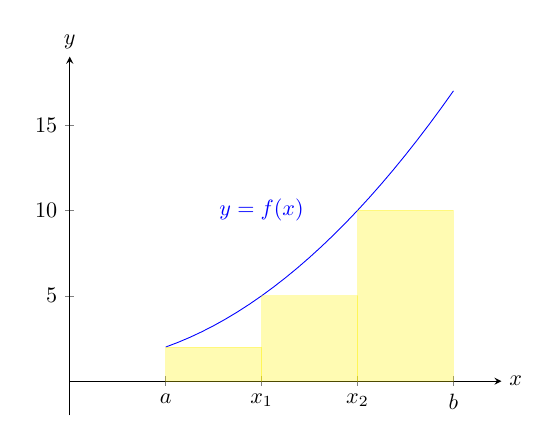
\begin{tikzpicture}[scale=0.8]
\begin{axis}[domain=1:4, xmin=0, xmax=4.5, ymax=19, ymin=-2, axis lines=middle, xlabel={\(x\)}, ylabel={\(y\)},
xlabel style={anchor=west}, ylabel style={anchor=south}, xtick={1,2,3,4}, xticklabels={\(a\),\(x_1\),\(x_2\),\(b\)}]
\addplot[blue]{x^2+1};
\node[blue] () at (2,10) {\(y=f(x)\)};
\pgfplotsinvokeforeach{1,2,3} {
\draw[yellow, fill, opacity=0.3] (#1,\fpeval{#1^2+1}) rectangle (\fpeval{#1+1},0);
}
\end{axis}
\end{tikzpicture}
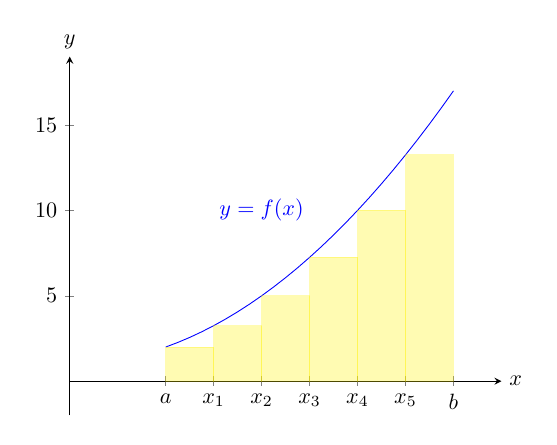
\begin{tikzpicture}[scale=0.8]
\begin{axis}[domain=1:4, xmin=0, xmax=4.5, ymax=19, ymin=-2, axis lines=middle, xlabel={\(x\)}, ylabel={\(y\)},
xlabel style={anchor=west}, ylabel style={anchor=south}, xtick={1,1.5,2,2.5,3,3.5,4}, xticklabels={\(a\),\(x_1\),\(x_2\),\(x_3\),\(x_4\),\(x_5\),\(b\)}]
\addplot[blue]{x^2+1};
\node[blue] () at (2,10) {\(y=f(x)\)};
\pgfplotsinvokeforeach{1,1.5,...,3.5} {
\draw[yellow, fill, opacity=0.3] (#1,\fpeval{#1^2+1}) rectangle (\fpeval{#1+0.5},0);
}
\end{axis}
\end{tikzpicture}
\end{center}
\item \emph{Lebesgue integral:} We partition the \(y\)-axis into finer and
finer pieces to approach to the area under curve.

\emph{More details:} First assume that the function \(f\) is nonnegative on
\([a,b]\). Let \(\Pi=\{y_0,y_1,y_2,\dotsc\}\) be a partition of the \(y\)-axis,
where \(0=y_0<y_1<y_2<\dotsb\). For each subinterval \([y_{k},y_{k+1}]\), let
\(A_k:=\{x\in[a,b]:y_k\le f(x)<y_{k+1}\}\). Then the \defn{lower Lebesgue sum}
is defined to be
\(\operatorname{LS}^{-}_{\Pi}(f)=\sum_{k=1}^{\infty}y_k\mu(A_k)\), where
\(\mu\) is a measure to be specified, e.g., Lebesgue measure. With a finer and
finer partition, the lower Lebesgue sum (sum of areas of rectangles below)
would approach to the area under curve (when the curve is ``sufficiently
nice'').
\begin{center}
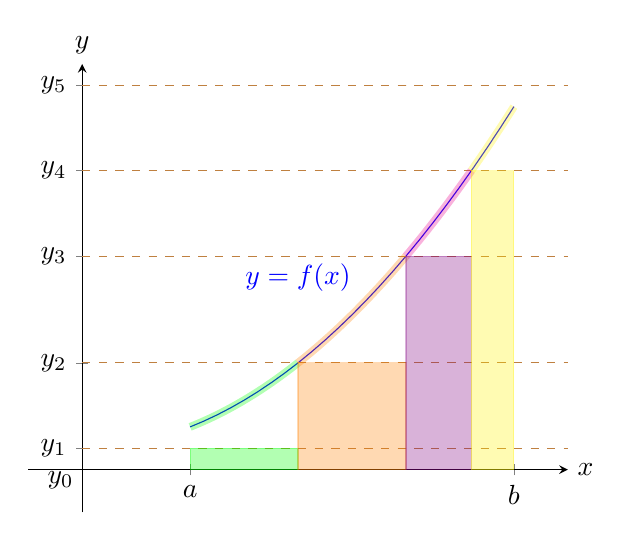
\begin{tikzpicture}
\begin{axis}[domain=1:4, xmin=-0.5, xmax=4.5, ymax=19, ymin=-2, axis lines=middle, xlabel={\(x\)}, ylabel={\(y\)},
xlabel style={anchor=west}, ylabel style={anchor=south}, xtick={1,4}, xticklabels={\(a\),\(b\)},
ytick={1,5,10,14,18}, yticklabels={\(y_1\), \(y_2\), \(y_3\), \(y_4\), \(y_5\)}]
\addplot[blue]{x^2+1};
\node[blue] () at (2,9) {\(y=f(x)\)};
\node[] () at (-0.2,-0.5) {\(y_0\)};
\addplot[domain=0:4.5, brown, dashed]{1};
\addplot[domain=0:4.5, brown, dashed]{5};
\addplot[domain=0:4.5, brown, dashed]{10};
\addplot[domain=0:4.5, brown, dashed]{14};
\addplot[domain=0:4.5, brown, dashed]{18};
\addplot[domain=1:2, green, opacity=0.3, line width=1mm]{x^2+1};
\draw[green, fill, opacity=0.3] (1,1) rectangle (2,0);
\addplot[domain=2:3, orange, opacity=0.3, line width=1mm]{x^2+1};
\draw[orange, fill, opacity=0.3] (2,5) rectangle (3,0);
\addplot[domain=3:3.606, magenta, opacity=0.3, line width=1mm]{x^2+1};
\draw[violet, fill, opacity=0.3] (3,10) rectangle (3.606,0);
\addplot[domain=3.606:4, yellow, opacity=0.3, line width=1mm]{x^2+1};
\draw[yellow, fill, opacity=0.3] (3.606,14) rectangle (4,0);
\end{axis}
\end{tikzpicture}
\end{center}
\end{itemize}
\item \label{it:lebesgue-int-def}\textbf{Definition of Lebesgue integral.}
As we are primarily discussing expectations here, we will focus on defining
Lebesgue integral of a \emph{random variable} \(X\) on a probability space
\((\Omega,\mathcal{F},\pr)\) (although it can be similarly defined for
measurable real-valued functions in general). The definition takes two steps:
\begin{enumerate}[label={(\arabic*)}] \item \emph{(definition for nonnegative
random variables)} For now, assume that \(0\le X(\omega)<\infty\) for all
\(\omega\in\Omega\). Let \(\Pi=\{y_0,y_1,y_2,\dotsc\}\) be a partition where
\(0=y_0<y_1<y_2<\dotsb\).  For each subinterval \([y_{k},y_{k+1}]\), let
\(A_k=\{\omega\in\Omega:y_k\le
X(\omega)<y_{k+1}\}=X^{-1}([y_k,y_{k+1}))\in\mathcal{F}\) (as \(X\) is a random
variable). Consider the lower Lebesgue sum
\(\operatorname{LS}^{-}_{\Pi}(X)=\sum_{k=1}^{\infty}y_k\prob{A_k}\).

Let \(\|\Pi\|\) be the maximal distance between the neighbouring partition
points in \(\Pi\). Then, the \defn{Lebesgue integral} is defined to be the
limit of the lower Lebesgue sum \(\operatorname{LS}^{-}_{\Pi}(X)\) as
\(\|\Pi\|\to 0\):
\[
\int_{\Omega}^{}X(\omega)\odif{\prob{\omega}}:=\lim_{\|\Pi\|\to 0}\operatorname{LS}^{-}_{\Pi}(X)
\footnote{Actually some technical details are omitted here (e.g., what does
``\(\lim_{\|\Pi\|\to 0}\)'' mean mathematically?), and the formal treatment of
Lebesgue integral is more involved (see STAT7610 for more details). But for our
purpose, it is enough to have basic understanding on Lebesgue integral above
and have some geometric intuition about it, e.g., the Lebesgue integral
\(\int_{\Omega}^{}c\odif{\prob{\omega}}\) can be geometrically viewed as the
area of rectangle with length \(\prob{\Omega}=1\) and height \(c\), which is
\(c\).},
\]
which is always nonnegative and could be \(\infty\).
\begin{note}
This notation is ``inspired'' by the previous expectation formula \(
\expv{X}=\sum_{\omega\in\Omega}^{}X(\omega)\prob{\{\omega\}}\) in the case with
countable \(\Omega\).
\end{note}

An alternative notation for the Lebesgue integral is \(\int_{\Omega}^{}X\odif{\pr}\).
\begin{center}
\begin{tikzpicture}
\begin{axis}[domain=0.8:4, xmin=-0.5, xmax=4.5, ymax=19, ymin=-4, axis y
line=middle, axis x line=none, xlabel={\(x\)}, ylabel={\(y\)}, xlabel
style={anchor=west}, ylabel style={anchor=south}, xtick={1,4},
xticklabels={\(a\),\(b\)}, ytick={0,2,5,10,14,18}, yticklabels={\(y_0\), \(y_1\), \(y_2\),
\(y_3\), \(y_4\), \(y_5\)}, samples=50]
\addplot[blue]{9+9*sin(1.8*deg(x-1))};
\node[blue] () at (3,17) {\(y=X(\omega)\)};
\addplot[domain=0:4.5, brown, dashed]{0};
\addplot[domain=0:4.5, brown, dashed]{2};
\addplot[domain=0:4.5, brown, dashed]{5};
\addplot[domain=0:4.5, brown, dashed]{10};
\addplot[domain=0:4.5, brown, dashed]{14};
\addplot[domain=0:4.5, brown, dashed]{18};
\addplot[green, opacity=0.3, domain=0.8:1.062, line width=1mm]{9+9*sin(1.8*deg(x-1))};
\addplot[green, opacity=0.3, domain=2.683:3.001, line width=1mm]{9+9*sin(1.8*deg(x-1))};
\addplot[orange, opacity=0.3, domain=1.062:1.327, line width=1mm]{9+9*sin(1.8*deg(x-1))};
\addplot[orange, opacity=0.3, domain=2.418:2.683, line width=1mm]{9+9*sin(1.8*deg(x-1))};
\addplot[violet, opacity=0.3, domain=1.327:2.418, line width=1mm]{9+9*sin(1.8*deg(x-1))};
\addplot[magenta, opacity=0.3, domain=3.001:3.240,, line width=1mm]{9+9*sin(1.8*deg(x-1))};
\addplot[yellow, opacity=0.3, domain=3.240:4,, line width=1mm]{9+9*sin(1.8*deg(x-1))};
\draw[green, fill, opacity=0.3] (0.8,5) rectangle (1.062,0);
\draw[green, fill, opacity=0.3] (2.683,5) rectangle (3.001,0);
\draw[orange, fill, opacity=0.3] (1.062,10) rectangle (1.327,0);
\draw[orange, fill, opacity=0.3] (2.418,10) rectangle (2.683,0);
\draw[violet, fill, opacity=0.3] (1.327,14) rectangle (2.418,0);
\draw[magenta, fill, opacity=0.3] (3.001,2) rectangle (3.240,0);
\draw[yellow, fill, opacity=0.3] (3.240,0) rectangle (4,0);
\draw[-Latex, ForestGreen] (2,-2) -- (0.9,0);
\draw[-Latex, ForestGreen] (2,-2) -- (2.8,0);
\node[ForestGreen] () at (2,-3) {\(y_2\prob{A_2}\)};
\draw[-Latex, orange] (3,-2) -- (1.15,0);
\draw[-Latex, orange] (3,-2) -- (2.5,0);
\node[orange] () at (3,-3) {\(y_3\prob{A_3}\)};
\draw[-Latex, violet] (1,-2) -- (1.85,0);
\node[violet] () at (1,-3) {\(y_4\prob{A_4}\)};
\draw[-Latex, magenta] (4,-2) -- (3.1,0);
\node[magenta] () at (4,-3) {\(y_1\prob{A_1}\)};
\end{axis}
\end{tikzpicture}
\end{center}
\emph{Some extensions:} (assuming \(X\) is allowed to take the value of \(\infty\))
\begin{itemize}
\item If \(\prob{\{\omega\in\Omega:X(\omega)=\infty\}}=0\) or
\(\prob{\{\omega\in\Omega:X(\omega)<0\}}=0\), then the Lebesgue integral turns
out to remain unchanged.
\begin{note}
This suggests that we indeed only require \(0\le X<\infty\) to hold with
probability \(1\).
\end{note}
\item If \(\prob{\{\omega\in\Omega:X(\omega)=\infty\}}>0\), then we \emph{define}
\(\int_{\Omega}^{}X(\omega)\odif{\prob{\omega}}:=\infty\).
\end{itemize}
\item \emph{(definition for general random variables)} Having the definition
for nonnegative random variables, we can define the Lebesgue integral for
general random variables through splitting them into \emph{positive parts} and
\emph{negative parts}. Given any random variable \(X\),
\begin{itemize}
\item the \defn{positive part} of \(X\) is given by
\(X^{+}(\omega)=\max\{X(\omega),0\}\) for all \(\omega\in\Omega\);
\item the \defn{negative part} of \(X\) is given by
\(X^{-}(\omega)=\max\{\rc{-}X(\omega),0\}\) for all \(\omega\in\Omega\).
\end{itemize}
Note that both \(X^{+}\) and \(X^{-}\) are nonnegative random variables. Also
we have \(X=X^{+}-X^{-}\) and \(|X|=X^{+}+X^{-}\).

In this general setting, the \defn{Lebesgue integral}
\(\int_{\Omega}^{}X(\omega)\odif{\prob{\omega}}\) is defined based on the
positive and negative parts.
\begin{itemize}
\item \emph{Case 1: \(\int_{\Omega}^{}X^{+}(\omega)\odif{\prob{\omega}}<\infty\) and
\(\int_{\Omega}^{}X^{-}(\omega)\odif{\prob{\omega}}<\infty\).}
We define
\[
\int_{\Omega}^{}X(\omega)\odif{\prob{\omega}}:=
\int_{\Omega}^{}X^{+}(\omega)\odif{\prob{\omega}}
-\int_{\Omega}^{}X^{-}(\omega)\odif{\prob{\omega}}.
\]
In this case, we also say that \(X\) is \defn{integrable}.
\item \emph{Case 2: \(\int_{\Omega}^{}X^{+}(\omega)\odif{\prob{\omega}}=\infty\) and
\(\int_{\Omega}^{}X^{-}(\omega)\odif{\prob{\omega}}<\infty\).}
We define
\[
\int_{\Omega}^{}X(\omega)\odif{\prob{\omega}}:=\infty.
\]
\item \emph{Case 3: \(\int_{\Omega}^{}X^{+}(\omega)\odif{\prob{\omega}}<\infty\) and
\(\int_{\Omega}^{}X^{-}(\omega)\odif{\prob{\omega}}=\infty\).}
We define
\[
\int_{\Omega}^{}X(\omega)\odif{\prob{\omega}}:=-\infty.
\]
\item \emph{Case 4: \(\int_{\Omega}^{}X^{+}(\omega)\odif{\prob{\omega}}=\infty\) and
\(\int_{\Omega}^{}X^{-}(\omega)\odif{\prob{\omega}}=\infty\).}
We leave \(\int_{\Omega}^{}X(\omega)\odif{\prob{\omega}}\) \emph{undefined}.
\end{itemize}
\end{enumerate}
Apart from the Lebesgue integral over the whole sample space \(\Omega\)
discussed above, we can also define the \defn{Lebesgue integral over a set
\(A\in\mathcal{F}\)} (where \(\mathcal{F}\) is a \(\sigma\)-algebra on
\(\Omega\)) as follows:
\[
\int_{A}^{}X(\omega)\odif{\prob{\omega}}=\int_{\Omega}^{}\indic_{A}(\omega)X(\omega)\odif{\prob{\omega}},
\]
where \(\indic_{A}\) denotes the indicator function.
\begin{note}
In a similar manner, the Lebesgue integral can be defined for measures other
than \(\pr\), e.g., the Lebesgue measure \(\lambda\), and similar notations
apply; see STAT7610 for more details.
\end{note}
\item \textbf{Relationship between Riemann and Lebesgue integral.} The Lebesgue
integral can indeed be viewed as a generalization to the Riemann integral, as
suggested by the following result.
\begin{proposition}[Comparison of Riemann and Lebesgue integrals]
\label{prp:compare-riemann-lebesgue-int}
Let \(f\) be a bounded function on \([a,b]\) with \(a<b\). Then:
\begin{enumerate}
\item The Riemann integral \(\int_{a}^{b}f(x)\odif{x}\) is defined (i.e., \(f\)
is \emph{Riemann integrable}) iff the set \(\{x\in [a,b]:\text{\(f\) is not
continuous at \(x\)}\}\) has Lebesgue measure zero (or in short: \(f\) is
continuous \emph{almost everywhere}; see \labelcref{it:ae-as-terms}).
\item If the Riemann integral \(\int_{a}^{b}f(x)\odif{x}\) is defined, then
\(f\) is Borel measurable and the Lebesgue integral
\(\int_{[a,b]}^{}f(x)\odif{\lambda(x)}\) is also defined. Furthermore, the
Riemann and Lebesgue integrals agree. \begin{note}
In view of this, sometimes we write \(\int_{[a,b]}^{}f(x)\odif{x}\) to denote
the common value of the Riemann and Lebesgue integrals.
\end{note}
\end{enumerate}
\end{proposition}
\begin{pf}
Omitted.
\end{pf}
\item \label{it:lebesgue-int-prop} \textbf{Properties of Lebesgue integral.}
The Lebesgue integral turns out to possess similar properties as the Riemann
integral. Let \(X\) and \(Y\) be random variables on a probability space
\((\Omega,\mathcal{F},\pr)\).

\begin{enumerate}
\item If \(X\) takes only finitely many values \(y_0,\dotsc,y_n\), then
\(\int_{\Omega}^{}X(\omega)\odif{\prob{\omega}}=\sum_{k=0}^{n}y_k\prob{X=y_k}\).
\item \emph{(integrability)} \(X\) is integrable iff
\(\int_{\Omega}^{}|X(\omega)|\odif{\prob{\omega}}<\infty\).
\item \emph{(monotonicity)} If \(\prob{X\le
Y}=\prob{\{\omega\in\Omega:X(\omega)\le Y(\omega)\}}=1\), and both
\(\int_{\Omega}^{}X(\omega)\odif{\prob{\omega}}\) and
\(\int_{\Omega}^{}Y(\omega)\odif{\prob{\omega}}\) are defined, then
\(\int_{\Omega}^{}X(\omega)\odif{\prob{\omega}}\le \int_{\Omega}^{}Y(\omega)\odif{\prob{\omega}}\).
\item If \(\prob{X=Y}=1\) and one of the integrals
\(\int_{\Omega}^{}X(\omega)\odif{\prob{\omega}}\) and
\(\int_{\Omega}^{}Y(\omega)\odif{\prob{\omega}}\) is defined, then the other is
also defined and \(\int_{\Omega}^{}X(\omega)\odif{\prob{\omega}}
=\int_{\Omega}^{}Y(\omega)\odif{\prob{\omega}}\)
\item \emph{(linearity)} If (i) \(\alpha\) and \(\beta\) are real constants and
\(X\) and \(Y\) are both integrable, or (ii) \(\alpha\) and \(\beta\) are
\emph{nonnegative} constants and \(X\) and \(Y\) are both \emph{nonnegative},
then \(\int_{\Omega}^{}(\alpha X(\omega)+\beta Y(\omega))\odif{\prob{\omega}}
=\alpha\int_{\Omega}^{}X(\omega)\odif{\prob{\omega}}+\beta\int_{\Omega}^{}Y(\omega)\odif{\prob{\omega}}
\).
\end{enumerate}
\begin{pf}
Due to the lack of formal definition of Lebesgue integral here, we shall omit
the proof; see STAT7610 for more details.
\end{pf}
\item\label{it:expv-prop} \textbf{Definition and properties of expectation.} With the knowledge of
Lebesgue integral, it is straightforward to define the concept of expectation.
Let \(X\) be a random variable on a probability space
\((\Omega,\mathcal{F},\pr)\). Then the \defn{expectation} of \(X\) is defined by
\[
\expv{X}:=\int_{\Omega}^{}X(\omega)\odif{\prob{\omega}}.
\]
It is well-defined if (i) \(X\) is integrable (equivalently:
\(\expv{|X|}=\int_{\Omega}^{}|X(\omega)|\odif{\prob{\omega}}<\infty\)), or (ii)
\(\prob{X\ge 0}=1\). For (i), we always have \(\expv{X}<\infty\). However, for
(ii) we may have \(\expv{X}=\infty\).

Since the expectation is essentially a Lebesgue integral, the properties for
Lebesgue integral in \labelcref{it:lebesgue-int-prop} still apply (just using
the notation ``\(\expv{\cdot}\)'' instead of ``\(\int\)''). But apart from them, we
also have some extra.

Let \(X\) be a random variable on a probability space
\((\Omega,\mathcal{F},\pr)\).
\begin{enumerate}
\item If \(X\) takes only finitely many values \(y_0,\dotsc,y_n\), then
\(\expv{X}=\sum_{k=0}^{n}y_k\prob{X=y_k}\).
\item \emph{(integrability)} \(X\) is integrable iff \(\expv{|X|}<\infty\).
\item \emph{(monotonicity)} If \(\prob{X\le Y}=1\) and both \(\expv{X}\) and
\(\expv{Y}\) are defined, then \(\expv{X}\le\expv{Y}\).
\item If \(\prob{X=Y}=1\) and one of the expectations \(\expv{X}\) and
\(\expv{Y}\) is defined, then the other is also defined and
\(\expv{X}=\expv{Y}\).
\item \emph{(linearity)} If (i) \(\alpha\) and \(\beta\) are real constants and
\(X\) and \(Y\) are both integrable, or (ii) \(\alpha\) and \(\beta\) are
\emph{nonnegative} constants and \(X\) and \(Y\) are both \emph{nonnegative}, then
\(\expv{\alpha X+\beta Y}=\alpha\expv{X}+\beta\expv{Y}\).
\item \emph{(Jensen's inequality)} If \(\varphi\) is a convex and real-valued function on \(\R\), and
\(\expv{|X|}<\infty\), then \(\varphi(\expv{X})\le\expv{\varphi(X)}\).
\end{enumerate}
\begin{pf}
Here we only prove the Jensen's inequality (based on the monotonicity and
linearity).
\begin{center}
\begin{tikzpicture}
\begin{axis}[domain=1:4, ymin=0, xtick={2.5}, ytick={1.25}, xticklabel={\(\expv{X}\)}, yticklabel={\(\varphi(\expv{X})\)}]
\addplot[blue]{(x-2)^2+1};
\node[blue] () at (2,1.5) {\(\varphi\)};
\addplot[ForestGreen]{x-1.25};
\draw[violet, fill] (2.5,1.25) circle [radius=0.7mm];
\node[ForestGreen] () at (2.5,0.5) {\(\ell(x)=ax+b\)};
\end{axis}
\end{tikzpicture}
\end{center}
Let \gc{\(\ell(x)=ax+b\)} denote a \emph{support line} of the convex function
\blc{\(\varphi\)} at \(x=\expv{X}\), i.e., a line that lies under the graph
of \(\varphi\) always and passes through the point
\((\expv{X},\varphi(\expv{X}))\).\footnote{The existence of support line is
guaranteed by the convexity of \(\varphi\). But here we will not delve into the
mathematical details about it.}

Then, we have \(a\orc{X(\omega)}+b\le\varphi(\orc{X(\omega)})\) for all
\(\omega\in\Omega\).  By monotonicity, we have
\(\expv{aX+b}\le\expv{\varphi(X)}\). Applying the linearity of the expectation
on the LHS (with \(\alpha=a, \beta=b, Y\equiv 1\)) gives
\(\ell(\expv{X})=a\expv{X}+b\le\expv{\varphi(X)}\). Since the line \(\ell\)
passes through \((\expv{X},\varphi(\expv{X}))\), we have
\(\ell(\expv{X})=\varphi(\expv{X})\), so we get
\(\varphi(\expv{X})\le\expv{\varphi(X)}\) as desired.
\end{pf}
\end{enumerate}
\subsection{Convergence Theorems}
\label{subsect:conv-thm}
\begin{enumerate}
\item\label{it:ae-as-terms} \textbf{Preliminary terms.} In \Cref{subsect:conv-thm}, we are going to
discuss several \emph{convergence theorems}, which give us conditions under
which we can ``interchange limit and integral''. We first introduce some
terminologies for describing the types of convergence to be investigated here.

Let \((\Omega,\mathcal{F},\mu)\) be a measure space (e.g., \(\mu\) may be the
Lebesgue measure \(\lambda\) or a probability measure \(\pr\)). Every set
\(N\in\mathcal{F}\) with \(\mu(N)=0\) is called a \defn{(\(\mu\)-)null set}. If
a statement holds for all \(\omega\in\Omega\setminus N\) where \(N\) is a null
set, then it is said to hold \defn{(\(\mu\)-)almost everywhere} (a.e.), or
\defn{(\(\mu\)-)almost surely} (a.s.) when \(\mu\) is a probability measure.

\item \textbf{Almost everywhere/surely convergence.} Let \(\{f_n\}\) be
a sequence of real-valued (Borel-)measurable functions on \(\R\), and let \(f\)
be another real-valued (Borel-)measurable function on \(\R\). Then we say that the sequence
\(\{f_n\}\) \defn{converges to \(f\) (\(\lambda\)-)almost everywhere}, denoted
by ``\(\lim_{n\to\infty}f_n=f\text{ (\(\lambda\)-)a.e.}\)'', if \(\lim_{n\to\infty}f_n(x)=f(x)\) for all \(x\in\R\setminus N\)
 where \(N\in\mathcal{B}\) is a (\(\lambda\)-)null set (\(\lambda\)
denotes the Lebesgue measure). \begin{note}
With the value \(x\) fixed, we can view \(\{f_n(x)\}\) as a real-valued
sequence with index \(n\), and ``\(\lim_{n\to\infty}f_n(x)=f(x)\)'' denote the
usual convergence of the sequence \(\{f_n(x)\}\) (to the fixed value \(f(x)\)),
i.e., the one you have seen in your previous calculus/analysis course.
\end{note}

In a similar way, we can define almost surely convergence for a sequence of
random variables. Let \(\{X_n\}\) be a sequence of random variables on a
probability space \((\Omega,\mathcal{F},\pr)\), and let \(X\) be another random
variable on the same probability space \((\Omega,\mathcal{F},\pr)\). Then we
say that the sequence \(\{X_n\}\) \defn{converges to \(X\) (\(\pr\)-)almost
surely}, denoted by ``\(\lim_{n\to\infty}f_n=f\text{ (\(\pr\)-)a.s.}\)'', if
\(\lim_{n\to\infty}X_n(\omega)=X(\omega)\) for all \(\omega\in\Omega\setminus
N\) where \(N\in\mathcal{F}\) is a (\(\pr\)-)null set.
\item \textbf{Monotone convergence theorem.} Now we are ready to state the
convergence theorems (without proofs as they are quite technical). For each of
them, we will state a version for real-valued measurable functions on \(\R\)
and a version for random variables (like what we did above).

The first convergence theorem is known as the \emph{monotone convergence
theorem} (MCT).

\begin{theorem}[Monotone convergence theorem]
\label{thm:mct}
\hfill
\begin{enumerate}
\item \emph{(for functions on \(\R\))}
Let \(\{f_n\}\) be a sequence of measurable real-valued functions on \(\R\) converging almost everywhere to
another measurable real-valued function \(f\) on \(\R\). If we have \(0\le f_1\le f_2\le\dotsb\) almost
everywhere, then
\[\lim_{n\to\infty}\int_{-\infty}^{\infty}f_n(x)\odif{x}
=\int_{-\infty}^{\infty}\lim_{n\to\infty}f_n(x)\odif{x}
=\int_{-\infty}^{\infty}f(x)\odif{x}.\]
\item \emph{(for random variables)}
Let \(\{X_n\}\) be a sequence of random variables converging almost surely to
another random variable \(X\). If we have \(0\le X_1\le X_2\le\dotsb\) almost
surely, then \[\lim_{n\to\infty}\expv{X_n}=\expv{\lim_{n\to\infty}X_n}=\expv{X},\] or more explicitly,
\[\lim_{n\to\infty}\int_{\Omega}^{}X_n(\omega)\odif{\prob{\omega}}
=\int_{\Omega}^{}\lim_{n\to\infty}X_n(\omega)\odif{\prob{\omega}}
=\int_{\Omega}^{}X(\omega)\odif{\prob{\omega}}.\]
\end{enumerate}
\end{theorem}
While the conditions involved in the MCT are ``\(0\le f_1\le f_2\le\dotsb\)
a.e.''\ or ``\(0\le X_1\le X_2\le\dotsb\) a.s.'', we can actually still apply
the MCT to more general sequences, by making the following observations:
\begin{itemize}
\item If \(c\le X_1\le X_2\le\dotsb\) a.s., then we have \(0\le X_1-c\le
X_2-c\le\dotsb\) a.s., so we can apply the MCT to the sequence \(\{X_n-c\}\).
\item If \(c\ge X_1\ge X_2\ge\dotsb\) a.s., then we have \(0\le c-X_1\le
c-X_2\le\dotsb\) a.s., so we can apply the MCT to the sequence \(\{c-X_n\}\).
\end{itemize}
\begin{note}
It is similar for the case with functions on \(\R\).
\end{note}
\item \textbf{Dominated convergence theorem.} Another convergence theorem to be
discussed here is the \emph{dominated convergence theorem} (DCT). Instead of
requiring \emph{monotonicity} as in MCT, here we require the functions/random
variables in the sequence to be bounded (``\underline{dominated}'') by a
function/random variable.

\begin{theorem}[Dominated convergence theorem]
\label{thm:dct}
\hfill
\begin{enumerate}
\item \emph{(for functions on \(\R\))}
Let \(\{f_n\}\) be a sequence of measurable real-valued functions on \(\R\)
converging almost everywhere to another measurable real-valued function \(f\)
on \(\R\). If we have \(|f_n|\le g\) almost everywhere for every \(n\in\N\),
where \(g\) is a function such that
\vc{\(\int_{-\infty}^{\infty}g(x)\odif{x}<\infty\)}, then
\[\lim_{n\to\infty}\int_{-\infty}^{\infty}f_n(x)\odif{x}
=\int_{-\infty}^{\infty}\lim_{n\to\infty}f_n(x)\odif{x}
=\int_{-\infty}^{\infty}f(x)\odif{x}.\]
\item \emph{(for random variables)}
Let \(\{X_n\}\) be a sequence of random variables converging almost surely to
another random variable \(X\). If we have \(|X_n|\le Y\) almost surely for
every \(n\in\N\), where \(Y\) is a random variable (defined on the same
probability space as others) with \vc{\(\expv{Y}<\infty\)}, then
\[\lim_{n\to\infty}\expv{X_n}=\expv{\lim_{n\to\infty}X_n}=\expv{X}.\]
\end{enumerate}
\end{theorem}
\end{enumerate}
\subsection{Computation of Expectations}
\begin{enumerate}
\item So far we have dealt with the concept of expectations theoretically. But
in practice, we are also interested in how we can \emph{compute} expectations.
Of course, you have already learnt computational formulas in your first course
in probability, namely:
\[
\expv{g(X)}=\begin{cases}
\sum_{k}^{}g(x_k)f(x_k)&\text{if \(X\) is discrete, taking countably many values \(x_1,x_2,\dotsc\)}, \\
\int_{-\infty}^{\infty}g(x)f(x)\odif{x}&\text{if \(X\) is continuous}.
\end{cases}
\]
Here we will investigate how our general and abstract definition of expectation
would get reduced to these formulas in these special cases. We start by stating
the following result.
\begin{proposition}
\label{prp:compute-expectation}
Let \(X\) be a random variable on a probability space
\((\Omega,\mathcal{F},\pr)\) and let \(g\) be a measurable function on \(\R\). Then
\[
\expv{g(X)}=\int_{\R}^{}g(x)\odif{\mu_X(x)},
\]
provided that \(\expv{g(X)}<\infty\).
\end{proposition}
In the case where \(X\) is discrete, taking countably many values
\(x_1,x_2,\dotsc\), the distribution measure \(\mu_X\) would then be given by
\(\mu_X(\{x_k\})=\prob{X=x_k}=f(x_k)\) for all \(k=1,2,\dotsc\), where \(f\) is
the mass function. This allows us to reduce the expression
\(\int_{\R}^{}g(x)\odif{\mu_X(x)}\) to \(\sum_{k}^{}g(x_k)f(x_k)\), which is
more familiar to us. For the case where \(X\) is continuous, there is a density
function \(f\) such that \(\mu_X(B)=\prob{X\in B}=\int_{B}^{}f(x)\odif{x}\) for all
\(B\in\mathcal{B}\). Based on this, it can be shown that
\(\int_{\R}^{}g(x)\odif{\mu_X(x)}
=\int_{-\infty}^{\infty}g(x)f(x)\odif{x}\)
(details omitted).
\end{enumerate}
\subsection{Change of Measure}
\label{subsect:change-of-meas}
\begin{enumerate}
\item We have now reached the last subsection in \Cref{sect:prob-theory}, which
is perhaps the most important one here also, due to its foundational role for
justifying the technique of \emph{risk-neutral pricing} that is heavily used in
financial economics (there we are changing the probability measure to the
\emph{risk-neutral measure}).

\item \label{it:change-meas-rv-z}\textbf{Changing measure through a random variable \(Z\).} The basic idea
of \emph{change of measure} is to introduce a random variable \(Z\) for
``distorting'' the probability measure. For illustration purpose, consider the
case where \(\Omega\) is countable with \(\prob{\{\omega\}}>0\) for every
\(\omega\in\Omega\). Suppose we would like to change the probability measure
\(\pr\) to a new probability measure \(\tpr\) via an introduction of a random
variable \(Z\). One natural way to do that is to define \(Z\) by
\(Z(\omega)=\tprob{\{\omega\}}/\prob{\{\omega\}}\) for all \(\omega\in\Omega\),
such that multiplying \(\prob{\{\omega\}}\) by \(Z(\omega)\) gives us the
``distorted'' probability \(\tprob{\{\omega\}}\), i.e.,
\(Z(\omega)\prob{\{\omega\}}=\tprob{\{\omega\}}\), for all \(\omega\in\Omega\).

However, difficult arises when \(\Omega\) is uncountable and
\(\prob{\{\omega\}}=\tprob{\{\omega\}}=0\) for all \(\omega\in\Omega\). In such
case, \emph{any} random variable \(Z\) would satisfy \(Z(\omega)\prob{\{\omega\}}=\tprob{\{\omega\}}\)
for all \(\omega\in\Omega\), since the equation is just saying
``\(0=0\)'', which is not meaningful and not what we want for describing how
the probability ``distortion'' should take place. Hence, instead of describing
the ``distorting'' on a ``per sample point \(\omega\)'' basis, we would describe
it on a ``per \emph{event}'' basis, as suggested by the following result.

\begin{proposition}
\label{prp:change-meas}
Let \((\Omega,\mathcal{F},\pr)\) be a probability space and let \(Z\) be an
almost surely nonnegative random variable with \(\expv{Z}=1\). Consider a
function \(\tpr\) defined by
\begin{equation}
\label{eq:change-of-measure}
\tprob{A}=\int_{A}^{}Z(\omega)\odif{\prob{\omega}}\quad\text{for every \(A\in\mathcal{F}\)}.
\end{equation}
Then \(\tpr\) is a probability measure on \(\mathcal{F}\).
\end{proposition}
\begin{pf}
\begin{enumerate}[label={(\arabic*)}]
\item For all \(A\in\mathcal{F}\), since we have \(\indic_{A}Z\ge 0\) almost
surely, by \labelcref{it:lebesgue-int-prop} we have \(\tprob{A}\ge 0\). \cmark
\item We have
\(\tprob{\Omega}=\int_{\Omega}^{}Z(\omega)\odif{\prob{\omega}}=\expv{Z}=1\).
\cmark \item Fix any pairwise disjoint events \(A_1,A_2,\dotsc\in\mathcal{F}\).
Let \(B_n:=\biguplus_{k=1}^{n}A_k\) for every \(n\in\N\) and
\(B_{\infty}:=\biguplus_{k=1}^{\infty}A_k\). Then \(B_n\nearrow\) and so we
have \(0\le\indic_{B_1}\le\indic_{B_2}\le\dotsb\), and hence \(0\le
\indic_{B_1}Z\le\indic_{B_2}Z\le\dotsb\) almost surely. Using the monotone
convergence theorem and the properties that for all \(\omega\in\Omega\),
\(\lim_{n\to\infty}\indic_{B_n}(\omega)=\indic_{B_{\infty}}(\omega)\) and
\(\indic_{B_n}(\omega)=\sum_{k=1}^{n}\indic_{A_k}(\omega)\), we have
\begin{align*}
\tprob{B_{\infty}}&=\int_{\Omega}^{}\indic_{B_{\infty}}(\omega)Z(\omega)\odif{\prob{\omega}}
=\int_{\Omega}^{}\lim_{n\to\infty}(\indic_{B_n}(\omega)Z(\omega))\odif{\prob{\omega}} \\
\overset{\text{(MCT)}}&{=}\lim_{n\to\infty}\int_{\Omega}^{}\indic_{B_n}(\omega)Z(\omega)\odif{\prob{\omega}}
=\lim_{n\to\infty}\int_{\Omega}^{}\indic_{B_n}(\omega)Z(\omega)\odif{\prob{\omega}} \\
&=\lim_{n\to\infty}\int_{\Omega}^{}\sum_{k=1}^{n}\indic_{A_k}(\omega)Z(\omega)\odif{\prob{\omega}}
\overset{\text{(linearity)}}{=}\lim_{n\to\infty}\sum_{k=1}^{n}\int_{\Omega}^{}\indic_{A_k}(\omega)Z(\omega)\odif{\prob{\omega}} \\
&=\lim_{n\to\infty}\sum_{k=1}^{n}\tprob{A_k}
=\sum_{k=1}^{\infty}\tprob{A_k}.\text{ \cmark}
\end{align*}
\end{enumerate}
\end{pf}
\item \textbf{Expectations after change of measure.} In \emph{risk-neutral
pricing}, after changing the probability measure to the \emph{risk-neutral
measure}, we would like to compute expectations under such probability measure.
In view of this, here we also study the effect of changing probability measure
on the expectations.

\begin{proposition}
\label{prp:exp-change-of-meas}
Let \((\Omega,\mathcal{F},\pr)\) be a probability space and let \(Z\) be an
almost surely nonnegative random variable with \(\expv{Z}=1\). Let \(\tpr\) be
defined as in \Cref{eq:change-of-measure}.
\begin{enumerate}
\item If \(X\) is a nonnegative random variable, then
\(\texpv{X}=\expv{XZ}\).
\item If \(Z>0\) almost surely, then \(\expv{Y}=\texpv{Y/Z}\) for every
nonnegative random variable \(Y\).
\end{enumerate}
\begin{note}
Here \(\texpv{\cdot}\) denotes the expectation under the probability measure
\(\tpr\), i.e., \(\texpv{X}=\int_{\Omega}^{}X(\omega)\odif{\tprob{\omega}}\).
\end{note}
\end{proposition}
\begin{pf}
First, note that (b) follows from (a) since in the case where \(Z>0\) and
\(Y\ge 0\) almost surely, the expression \(Y/Z\) can be defined (ignoring those
\(\omega\)'s where \(Z(\omega)=0\) would not affect the calculation of
expectation) and is almost surely nonnegative, so (b) follows by setting
\(X=Y/Z\) in (a). So we will only prove (a) in the following.

We will utilize a proof strategy known as the \emph{standard machine}, which is
a standard argument for proving results in measure theory. The \defn{standard
machine} takes four steps, which show the desired result holds for larger and
larger classes of functions: (1) indicator functions \faIcon{arrow-right} (2)
\defn{simple functions} (i.e., linear combinations of finitely many indicator
functions of pairwise disjoint sets) \faIcon{arrow-right} (3) nonnegative
random variables \faIcon{arrow-right} (4) general random variables.
As the results here are for nonnegative random variables, we only need to
perform the first three steps here. (We can also perform the step 4 to extend
the results to general random variables; see the remark afterwards.)

\emph{Step 1: Indicator functions.} For all \(A\in\mathcal{F}\), we have
\[
\texpv{\vc{\indic_{A}}}=\tprob{A}=\int_{\Omega}^{}\indic_{A}(\omega)Z(\omega)\odif{\omega}
=\expv{\vc{\indic_{A}}Z}.
\]
\emph{Step 2: Simple functions.} Fix any pairwise disjoint events
\(A_1,\dotsc,A_n\in\mathcal{F}\), and any constants \(c_1,\dotsc,c_n\in\R\). Then
\[
\texpv{\vc{\sum_{i=1}^{n}c_i\indic_{A_i}}}
=\sum_{i=1}^{n}c_i\texpv{\indic_{A_i}}
\overset{\text{(step 1)}}{=}\sum_{i=1}^{n}c_i\expv{\indic_{A_i}Z}
=\expv{\left(\vc{\sum_{i=1}^{n}c_i\indic_{A_i}}\right)Z}.
\]
\emph{Step 3: Nonnegative random variables.} We will use the fact that, given
any nonnegative random variable \(X\), there exists a sequence of nonnegative
simple functions \(\{X_n\}\) such that \(0\le X_1\le X_2\le\dotsb\le X\) a.s.\ and
\(\lim_{n\to\infty}X_n=X\) a.s. (loosely speaking, they are approaching to
\(X\) ``from below''). By monotone convergence theorem, we have
\[
\texpv{X}=\texpv{\lim_{n\to\infty}X_n}
=\lim_{n\to\infty}\texpv{X_n}
\overset{\text{(step 2)}}{=}\lim_{n\to\infty}\expv{X_nZ}
=\expv{\lim_{n\to\infty}(X_nZ)}
=\expv{XZ}.
\]
\end{pf}

\begin{remark}
\item Given any general random variable \(X\) that may not be nonnegative, we can
write \(X=X^{+}-X^{-}\) and apply (a) by \(\texpv{X}
=\texpv{X^{+}}-\texpv{X^{-}}
\overset{\text{(a)}}{=}\expv{X^{+}Z}-\expv{X^{-}Z}\), as long as it does not
result in ``\(\infty-\infty\)''.
\item Similarly for (b), we can apply it for every general random variable \(Y\)
through writing \(Y=Y^+-Y^-\): \(\expv{Y}=\texpv{Y^{+}/Z}-\texpv{Y^{-}/Z}\),
again as long as it does not result in ``\(\infty-\infty\)''.
\end{remark}
\item \textbf{Equivalent probability measures.} Let \(\Omega\) be nonempty and
\(\mathcal{F}\) be a \(\sigma\)-algebra on \(\Omega\). Then two probability
measures \(\pr\) and \(\tpr\) on \((\Omega,\mathcal{F})\) are called
\defn{equivalent} if we have \(\prob{A}=0\) iff \(\tprob{A}=0\), i.e., they
assign zero probability to \emph{exactly} the same collection of events in
\(\mathcal{F}\).
\begin{note}
While equivalent probability measures agree on which events in \(\mathcal{F}\)
have zero probability, they can still differ a lot on the probability
assignments for events with positive probability.
\end{note}

The following result provides a sufficient condition for two probability
measures to be equivalent.
\begin{proposition}
\label{prp:z-positive-equiv-prob}
Let \((\Omega,\mathcal{F},\pr)\) be a probability space and let \(Z\) be an
almost surely \rc{\emph{positive}} random variable with \(\expv{Z}=1\). Let
\(\tpr\) be defined as in \Cref{eq:change-of-measure}. Then, the two
probability measures \(\pr\) and \(\tpr\) are equivalent.
\end{proposition}
\begin{pf}
Fix any \(A\in\mathcal{F}\) with \(\prob{A}=0\). Then we have \(\indic_{A}Z=0\)
\(\pr\)-almost surely. Hence,
\(\tprob{A}=\int_{\Omega}^{}\indic_{A}(\omega)Z(\omega)\odif{\prob{\omega}}=\int_{\Omega}^{}0\odif{\prob{\omega}}=0\).

Conversely, fix any \(B\in\mathcal{F}\) with \(\tprob{B}=0\). Then we have
\(\indic_{B}/Z=0\) \(\tpr\)-almost surely. Hence,
\(\prob{B}=\expv{\indic_{B}}\overset{\text{(\Cref{prp:exp-change-of-meas})}}{=}\texpv{\indic_{B}/Z}=0\).
\end{pf}
\item \textbf{Radon-Nikodym theorem and Radon-Nikodym derivatives.}
The \emph{Radon-Nikodym theorem} is a theoretical result that guarantees the
existence of a random variable \(Z\) satisfying \Cref{eq:change-of-measure}
given two \emph{equivalent} probability measures.

\begin{theorem}[Radon-Nikodym]
\label{thm:radon-nikodym}
Let \(\pr\) and \(\tpr\) be equivalent probability measures on a measurable
space \((\Omega,\mathcal{F})\). Then there exists an almost surely
\emph{positive} random variable \(Z\) with \(\expv{Z}=1\) such that
\[
\tpr(A)=\int_{A}^{}Z(\omega)\odif{\prob{\omega}}\quad\text{for every \(A\in\mathcal{F}\)}.
\]
\end{theorem}
\begin{pf}
Omitted.
\end{pf}

Inspired by
\(\tpr(A)=\int_{\Omega}^{}\indic_{A}\odif{\tprob{\omega}}=\int_{A}^{}1\odif{\tprob{\omega}}\)
and the Radon-Nikodym theorem, we may write \(
Z(\omega)=:\odif{\tprob{\omega}}/\odif{\prob{\omega}}\) for all
\(\omega\in\Omega\), as a mnemonic device. (This looks somewhat similar to the
equation ``\( Z(\omega)=\tprob{\{\omega\}}/\prob{\{\omega\}}\)'' in
\labelcref{it:change-meas-rv-z}.) Indeed, such random variable \(Z\) in the
Radon-Nikodym theorem is known as the \defn{Radon-Nikodym derivative of
\(\tpr\) with respect to \(\pr\)}, which is often denoted by \(
\odif{\tpr}/\odif{\pr}\).
\end{enumerate}
